%% Mathematics 1b -- Problem Set 3
%% Compile with: pdflatex ps03.tex
\documentclass[11pt]{article}

\usepackage[margin=1in]{geometry}
\usepackage{amsmath}
\usepackage{amssymb}
\usepackage{graphicx}
\usepackage{math1b}          % \dd  \abs  \problem  \hint

\title{Mathematics 1b \\ Problem Set 3}
\author{}
\date{Due Friday, 2 October}

\begin{document}
\maketitle

\problem{1}

The function $\sin(x^{2})$ has no elementary antiderivative, so the integral
\[
  \int_{0}^{\pi} \sin(x^{2}) \dd{x}
\]
cannot be evaluated by any of the techniques in Chapter 7. It can still be
estimated to whatever accuracy you need.

\begin{figure}[htbp]
  \centering
  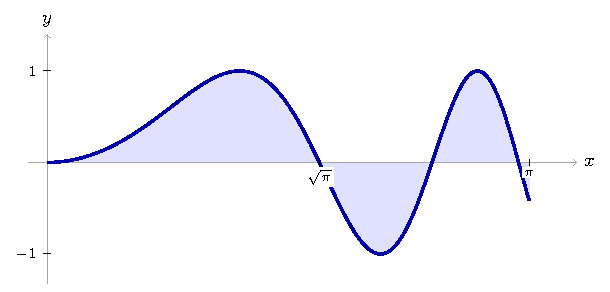
\includegraphics[width=0.58\textwidth]{figures/fresnel-curve.pdf}
  \caption{The graph of $y = \sin(x^{2})$ on $[0, \pi]$. The shaded region is
    the quantity you are estimating in part (c). The oscillation tightens as
    $x$ grows, because the argument grows like $x^{2}$.}
  \label{fig:fresnel}
\end{figure}

\begin{enumerate}
  \item Write the Maclaurin series for $\sin u$, then substitute $u = x^{2}$
        to obtain a power series for $\sin(x^{2})$.
  \item Integrate your series term by term to obtain a series whose sum is
        $\int_{0}^{\pi} \sin(x^{2}) \dd{x}$.
  \item The series in part (b) alternates. Use that fact to estimate the
        integral to within $0.01$, and say how many terms you needed.
\end{enumerate}

\hint{For an alternating series whose terms decrease in absolute value to
zero, the error after $n$ terms is no larger than the first omitted term.}

\problem{2}

Evaluate each of the following integrals.

\begin{enumerate}
  \item $\displaystyle \int x \sqrt{1 + x^{2}} \dd{x}$
  \item $\displaystyle \int_{0}^{1} \frac{2x}{1 + x^{2}} \dd{x}$
  \item $\displaystyle \int \frac{\cos(\ln x)}{x} \dd{x}$
\end{enumerate}

\hint{Each becomes elementary after a single substitution. For part (c), try
$u = \ln x$.}

\problem{3}

\begin{figure}[htbp]
  \centering
  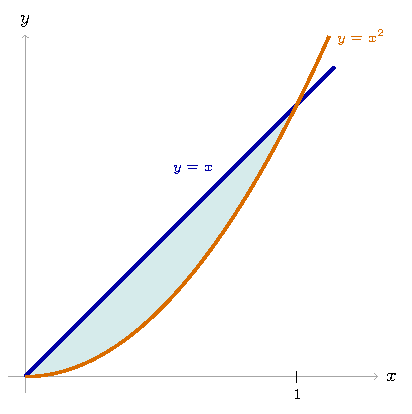
\includegraphics[width=0.42\textwidth]{figures/region-between-curves.pdf}
  \caption{The region bounded by $y = x$ and $y = x^{2}$ between their two
    points of intersection.}
  \label{fig:region}
\end{figure}

\begin{enumerate}
  \item Find the two points where $y = x$ and $y = x^{2}$ meet, and set up an
        integral for the area of the shaded region in Figure~\ref{fig:region}.
  \item Evaluate it.
  \item Evaluate $\displaystyle \int_{0}^{1} x e^{-x} \dd{x}$ using
        integration by parts, and explain in one sentence why substitution
        alone will not work here.
  \item Show that $\abs{\int_{0}^{1} x e^{-x} \dd{x}} < \tfrac{1}{2}$ without
        using your answer to part (c).
\end{enumerate}

\end{document}
